\documentclass[a4paper,14pt]{extarticle}
\usepackage[utf8]{inputenc}
\usepackage[legalpaper, portrait, margin=1in]{geometry}
\usepackage{enumitem}
\usepackage{graphicx}


\title{CS 156a Bonus Exercise}
\author{Cason Shepard}
\date\today

\begin{document}
\maketitle

\section{Classifying digits with NN’s}
\subsection*{1.3}
When The number of hidden units is varied, the following accuracy and loss graphs for the training program are generated.\\
\begin{center}
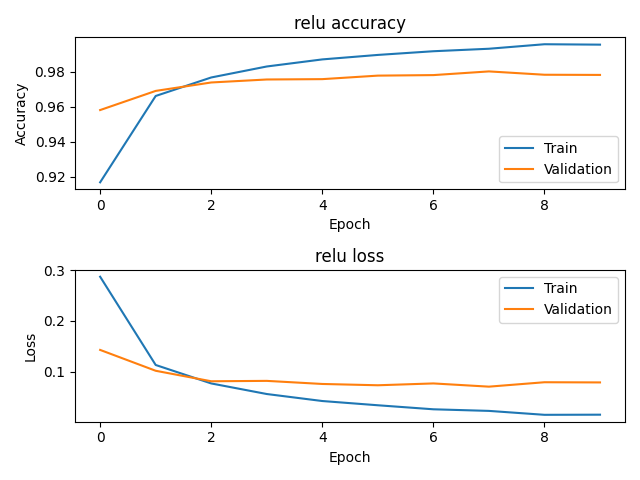
\includegraphics[width=400]{Figure_1_200_100_original.png}\\
This is the original accuracy/loss graphs using hidden layers of 200 and 100 units.\\Total trainable parameters: 178,110\\
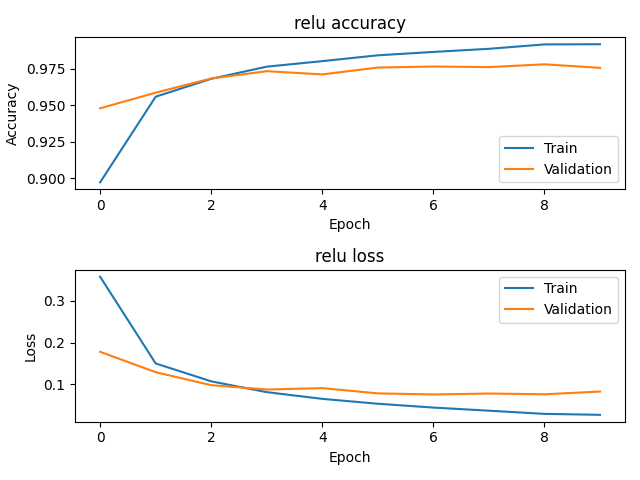
\includegraphics[width=400]{Figure_1_100_50.png}\\
This is the accuracy/loss graphs using hidden layers of 100 and 50 units.\\Total trainable parameters: 84,060\\
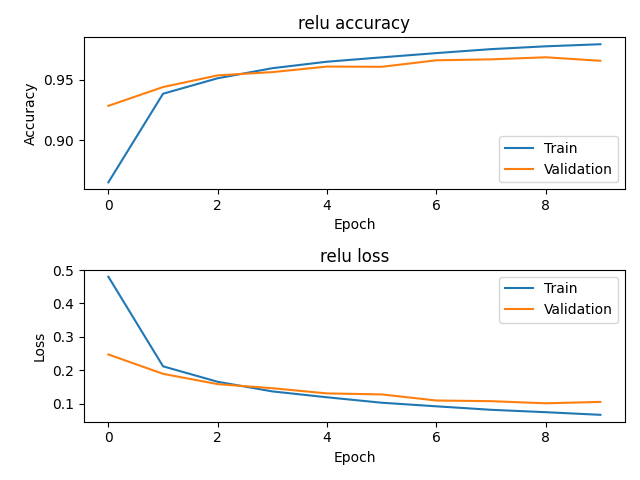
\includegraphics[width=400]{Figure_1_50_25.png}\\
This is the accuracy/loss graphs using hidden layers of 50 and 25 units.\\Total trainable parameters: 40,785
\end{center}
\textbf{I estimate that the smallest number of parameters to achieve $97\%$ accuracy is around 80,000.}
\subsection*{1.4}
In the following graphs, the REGULARIZATION parameter was varied and the \textit{ReLU} accuracy/loss was plotted.
\begin{center}
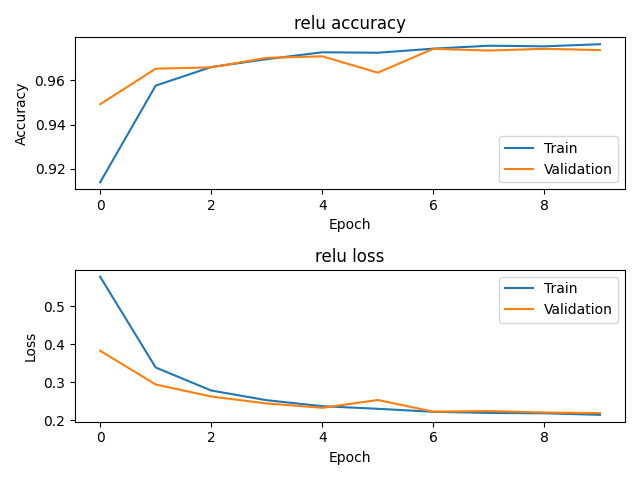
\includegraphics[width=400]{Figure_1_lambda_001.png}\\
This is the accuracy/loss plot for $\lambda = 0.001$.
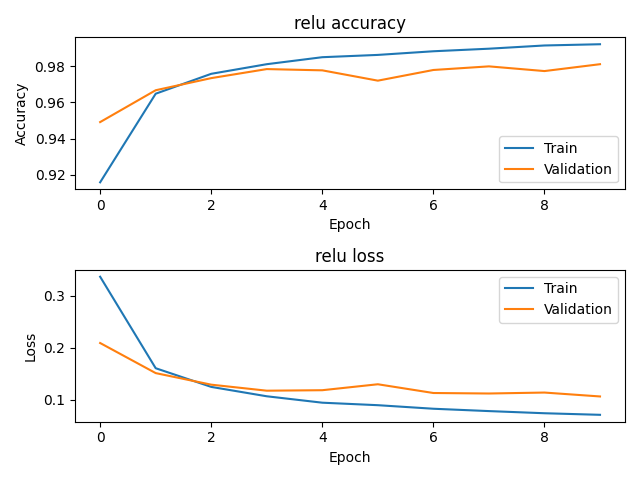
\includegraphics[width=400]{Figure_1_lambda_0001.png}\\
This is the accuracy/loss plot for $\lambda = 0.0001$. \textbf{This graph is most similar to the neural network I implemented above with hidden layers of 100 and 50 units respectively.}
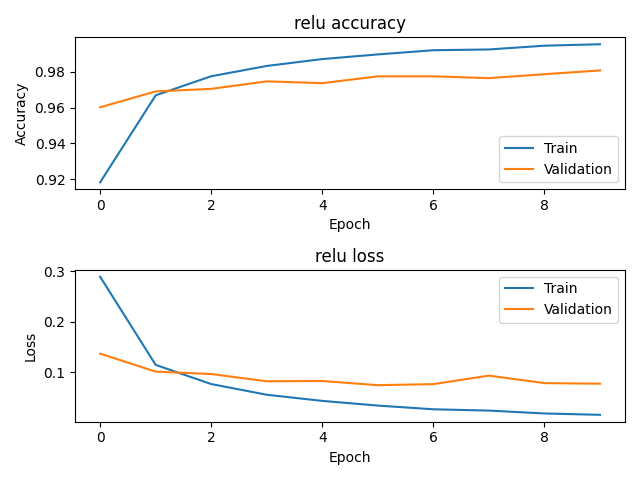
\includegraphics[width=400]{Figure_1_lambda_000001.png}\\
This is the accuracy/loss plot for $\lambda = 0.000001$.
\end{center}
\subsection*{1.5}
In the following plots, the \textit{tanh} activation function was used.  
\begin{center}
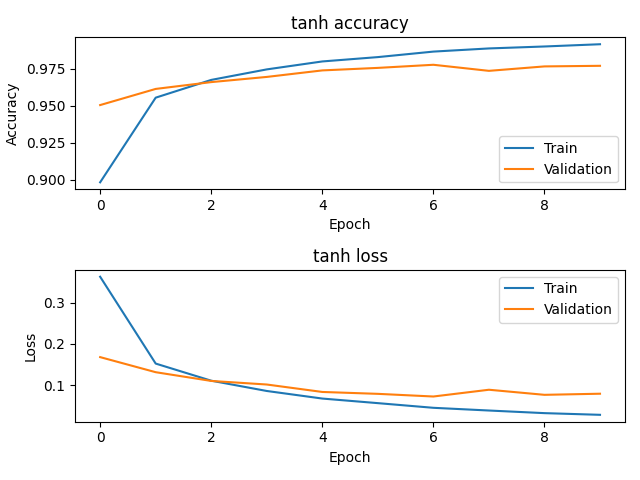
\includegraphics[width=400]{tanh_learn_100_50.png}\\
In this plot, the \textit{tanh} activation function was used with the original 100 and 50 unit hidden neural network layers. \textbf{Comparing this to the \textit{ReLU} function used over 100 and 50 unit hidden layers, we can see that the \textit{tanh} function converges faster than \textit{ReLU}.}
\end{center}
\subsection*{1.6}
The highest validation accuracy i was able to achieve was with an activation of \textit{tanh}, $\lambda = 10^{-7}$, and only a single hidden layer of 200 units. Validation accuracy was 0.9807.
\subsection*{1.7}
\begin{center}
Dense Neural Net\\
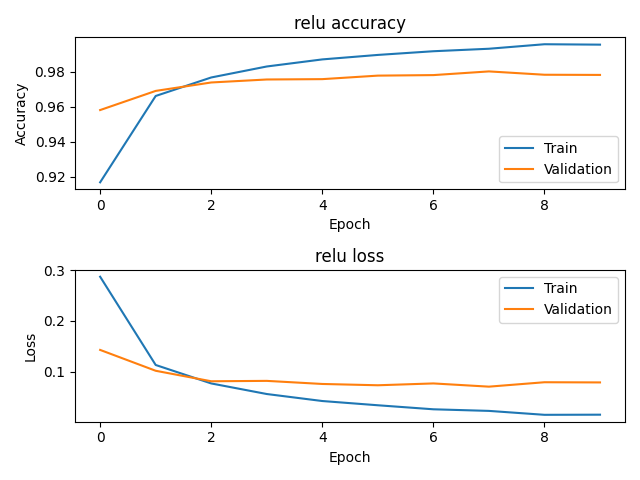
\includegraphics[width=300]{Figure_1_200_100_original.png}\\
Total Parameters: 178,110\\
Validation loss: 0.0760\\
Validation accuracy: 0.9790\\\\
\end{center}
\begin{center}
Convolutional Neural Net\\
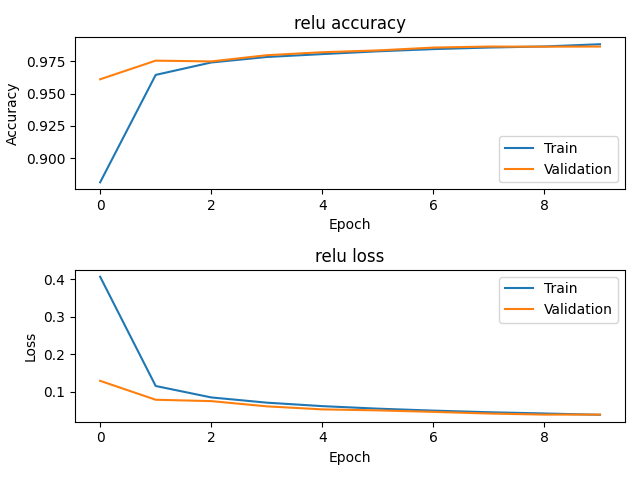
\includegraphics[width=300]{relu_learn_c.png}\\
Total Parameters: 7240\\
Validation loss: 0.0391\\
Validation accuracy: 0.9863\\
\end{center}
\textbf{The convolutional neural net had a higher validation accuracy and a lower validation loss than the dense neural network. Furthermore, the convolutional network had less parameters.}
\newpage
\section{Generative Adversarial Network}
\subsection*{2.2}
\begin{center}
    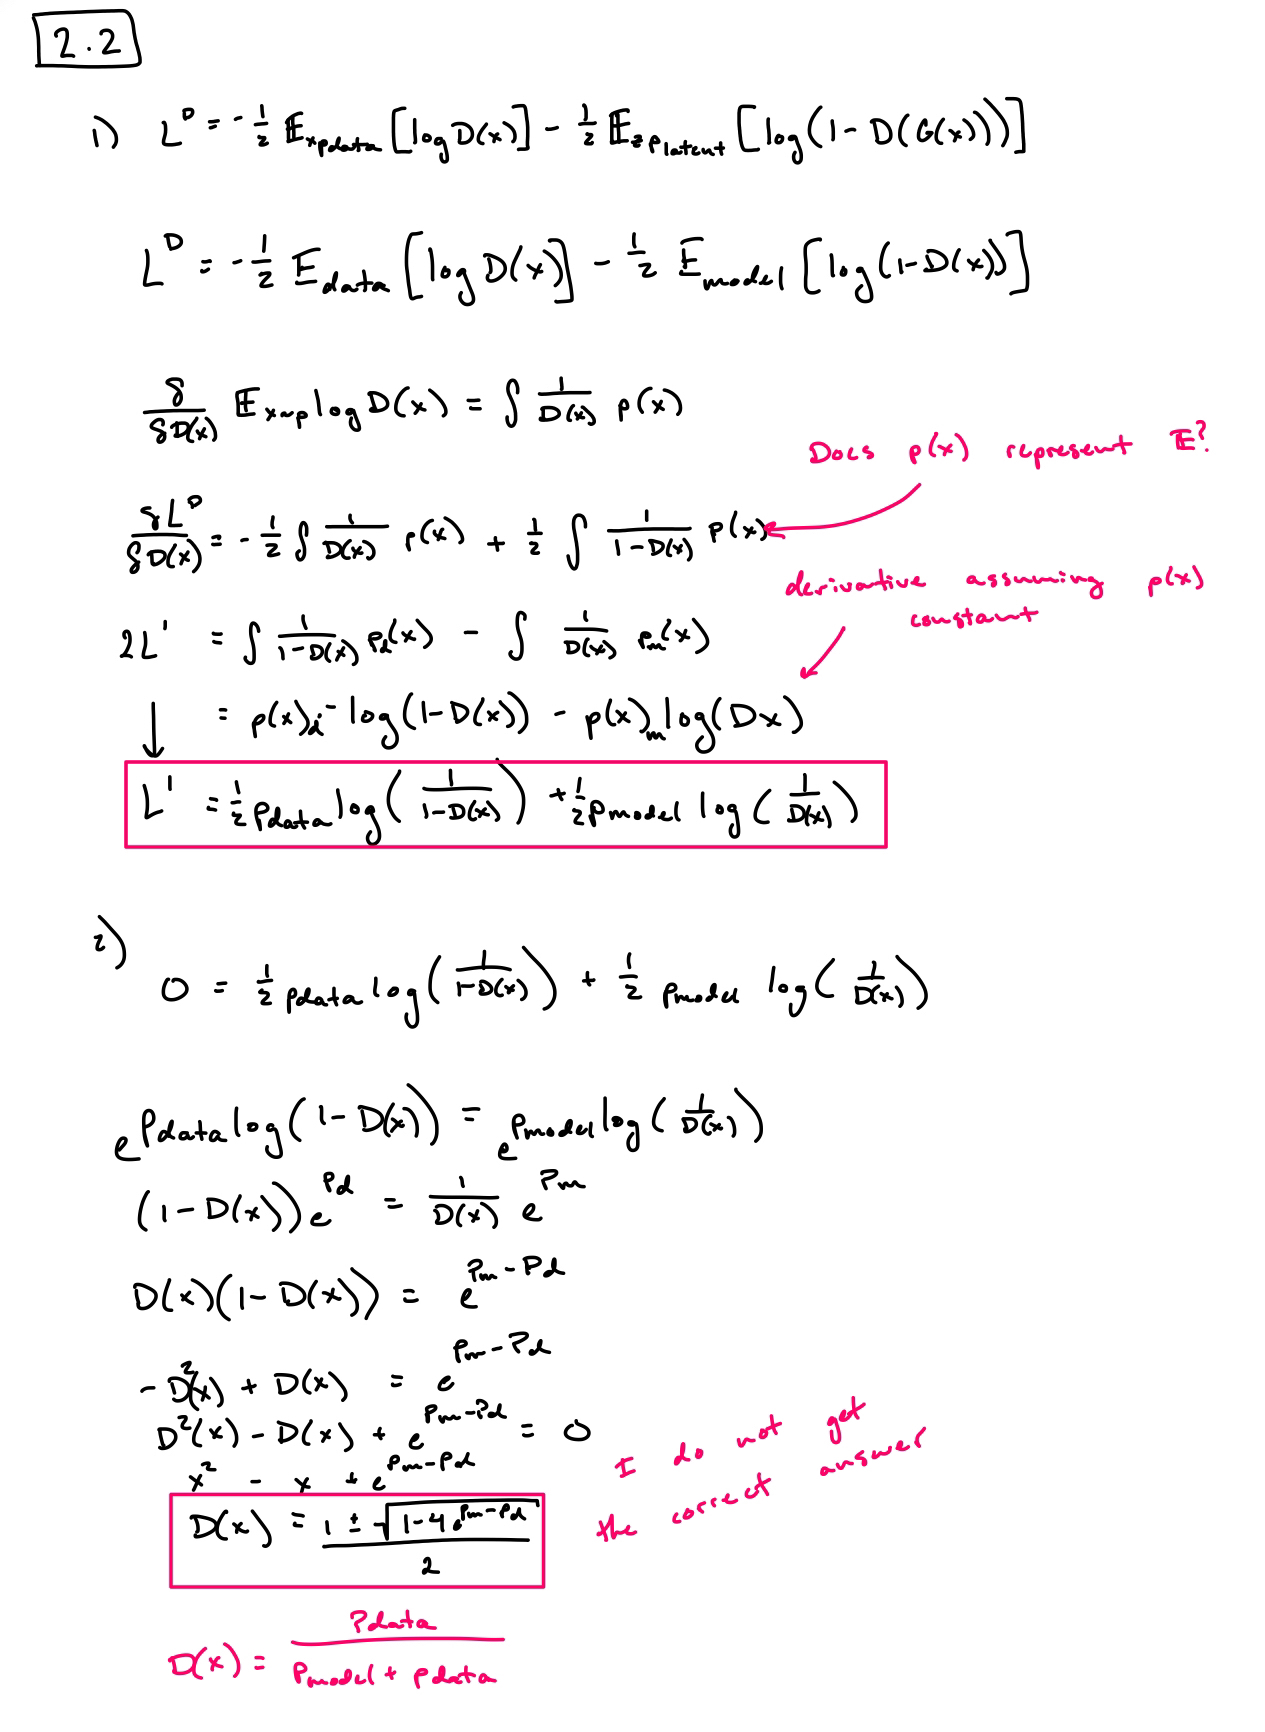
\includegraphics[width=450]{GAN_cs156Bonus_2.2.png}
\end{center}
\textbf{3)} This makes sense, as the discriminator should be determined as a combination of the target data and the model of this data. As far as why D(x) is formulated this way, I am unsure.
\subsection*{2.4}
The training process seemed to be very efficient, as epochs 1-10 generated very blurry images, but 20-50 began to produce more clear numbers. Past those, the generated images didn't seem to change too much as the epoch number grew. There seemed to be an accuracy threshold that was reached and then the accuracy did not increase more after that.\\\\
Mode collapse is when the generator begins to output the same thing many times. In this situation, the discriminator should be able to recognize this and adjust to reject these repeated outputs. The collapse happens when the generator learns to optimize around the discriminator, so the discriminator stops affecting the output.\\\\
I think the GAN provided avoids this by alternating between training of the discriminator and generator. That way the discriminator is forced to change after each generator change, thus, avoiding mode collapse.
\newpage
\section{Feedback}
I thought this mini project was enjoyable. Part 1 I ran locally in Windows Powershell, while Part 2 I ran on a Google Colab Notebook. I enjoyed using Powershell to run the scripts and edit them. I wish we could do more of this. Part 1 was slightly repetitive and it got tricky to decipher the axis on the graphs when trying to see if two graphs were similar. I also wish we got more explanation of what the given GAN was doing. 
\end{document}
